\chapter{O coração e o sangue}\label{ch:g4:heart-and-blood}

Aperte dois dedos --- não o polegar --- na parte de dentro do seu
\omterm{prop:g4:heart-and-blood:pulse}{pulso}, abaixo da base do polegar, e espere. Pronto: uma batidinha
firme, de novo e de novo, mais ou menos uma vez por segundo. Essa
\omterm{def:g4:heart-and-blood:heart}{batida} é o seu \omterm{def:g4:heart-and-blood:heart}{coração} trabalhando, sentido de longe. Ele bate desde
antes de você nascer, e é o motor do serviço de entregas do corpo.

\section{O sangue, o serviço de entregas do corpo}

\begin{proposition}[O que o sangue transporta]\label{prop:g4:heart-and-blood:carries}
O \emph{sangue}\index{sangue} é um líquido que chega a todos os
cantos do corpo, e é o transportador do corpo:
\begin{itemize}
  \item no \omterm{def:g4:journey-of-food:tract}{intestino delgado}, ele recolhe os \emph{\omterm{def:g4:journey-of-food:digestion}{nutrientes}}
        (\cref{prop:g4:journey-of-food:absorb});
  \item nos pulmões, ele recolhe o \emph{oxigênio}
        (\cref{prop:g4:breathing:exchange});
  \item ele entrega os dois a todas as partes do corpo --- \omterm{def:g3:bones-and-muscles:muscle}{músculos},
        cérebro, \omterm{def:g3:bones-and-muscles:skeleton}{ossos}, \omterm{def:g1:the-five-senses:sense}{pele};
  \item na volta, ele leva embora os resíduos, entregando o gás
        carbônico aos pulmões para ser expirado.
\end{itemize}
\end{proposition}
\admitted

\begin{example}[Uma rodada de entregas]\label{ex:g4:heart-and-blood:round}
Siga uma gota de \omterm{prop:g4:journey-of-food:absorb}{sangue}: ao passar pelos pulmões ela fica vermelha
viva, carregada de oxigênio; o \omterm{def:g4:heart-and-blood:heart}{coração} a manda para fora; num
\omterm{def:g3:bones-and-muscles:muscle}{músculo} da \omterm{def:g1:my-body:parts}{perna} em plena corrida ela entrega o oxigênio e os
\omterm{def:g4:journey-of-food:digestion}{nutrientes}, recolhe o gás carbônico e escurece; de volta ao \omterm{def:g4:heart-and-blood:heart}{coração},
ela é mandada aos pulmões para descarregar e recarregar --- e sair
de novo. Uma rodada completa leva bem menos de um minuto.
\end{example}

\begin{definition}[Vasos sanguíneos]\label{def:g4:heart-and-blood:vessels}
O \omterm{prop:g4:journey-of-food:absorb}{sangue} viaja em tubos chamados \emph{vasos sanguíneos}\index{vaso
sanguíneo}: largos ao sair e ao entrar no \omterm{def:g4:heart-and-blood:heart}{coração}, ramificando-se
cada vez mais finos --- até vasos da espessura de um fio de cabelo
que se enfiam entre as partes do corpo, onde as entregas são feitas.
Enfileirados ponta a ponta, os vasos de um corpo se estenderiam por
dezenas de milhares de quilômetros.
\end{definition}

\begin{remark}[Ver os vasos]\label{rem:g4:heart-and-blood:see}
Olhe a parte de baixo do seu \omterm{prop:g4:heart-and-blood:pulse}{pulso}: linhas azuladas debaixo da \omterm{def:g1:the-five-senses:sense}{pele}
--- \omterm{def:g4:heart-and-blood:vessels}{vasos sanguíneos} a caminho de volta ao \omterm{def:g4:heart-and-blood:heart}{coração}. Um \omterm{def:g1:my-body:joint}{joelho}
ralado mostra a outra ponta da rede: até o corte mais fininho acha
\omterm{prop:g4:journey-of-food:absorb}{sangue}, porque os \omterm{def:g4:heart-and-blood:vessels}{vasos} mais finos estão em toda parte.
\end{remark}

\section{O coração, a bomba}

\begin{definition}[O coração]\label{def:g4:heart-and-blood:heart}
O \emph{coração}\index{coração} é um \omterm{def:g3:bones-and-muscles:muscle}{músculo} oco, mais ou menos do
tamanho do \omterm{def:g1:my-body:joint}{punho} fechado do dono, no meio do peito, atrás da caixa
torácica. Ao apertar --- uma \emph{batida}\index{batida do coração}
--- ele empurra o \omterm{prop:g4:journey-of-food:absorb}{sangue} pelos \omterm{def:g4:heart-and-blood:vessels}{vasos}. Ele tem dois lados: o lado
direito bombeia o \omterm{prop:g4:journey-of-food:absorb}{sangue} até os \emph{pulmões} para carregar
oxigênio; o lado esquerdo bombeia o \omterm{prop:g4:journey-of-food:absorb}{sangue} rico em oxigênio para o
\emph{corpo inteiro}.
\end{definition}

\begin{omfigure}
\begin{tikzpicture}[scale=0.95]
  % heart: two chambers schematic
  \draw[thick, fill=omThm!10] (0,0)
    .. controls (-1.5,0.9) and (-1.3,2.3) .. (-0.35,2.3)
    .. controls (-0.05,2.3) and (0.0,2.15) .. (0.0,2.05)
    .. controls (0.0,2.15) and (0.05,2.3) .. (0.35,2.3)
    .. controls (1.3,2.3) and (1.5,0.9) .. (0,0);
  \draw[thick] (0,2.05) -- (0,0.35);
  \node[font=\small, align=center] at (-0.55,1.45) {lado\\ direito};
  \node[font=\small, align=center] at (0.55,1.45) {lado\\ esquerdo};
  % arrows: right side to lungs
  \draw[->, very thick, omDef] (-0.55,2.3) .. controls (-0.8,3.0)
    .. (-1.9,3.2)
    node[left, font=\small, omDef, align=center] {para os pulmões:\\ carregar oxigênio};
  \draw[->, very thick, omDef!50] (-3.0,2.2) .. controls (-2.0,2.0)
    .. (-1.15,1.6);
  \node[font=\small, omDef!80, align=center, left] at (-3.05,2.2)
    {de volta do\\ corpo};
  % arrows: left side to body
  \draw[->, very thick, omThm] (0.55,2.3) .. controls (0.8,3.0)
    .. (1.9,3.2)
    node[right, font=\small, omThm, align=center] {para o corpo inteiro:\\ entregar oxigênio};
  \draw[->, very thick, omThm!50] (3.0,2.2) .. controls (2.0,2.0)
    .. (1.15,1.6);
  \node[font=\small, omThm!80, align=center, right] at (3.05,2.2)
    {de volta dos\\ pulmões};
\end{tikzpicture}

{\small Os dois lados do \omterm{def:g4:heart-and-blood:heart}{coração}: o lado direito manda o \omterm{prop:g4:journey-of-food:absorb}{sangue} aos
pulmões atrás de oxigênio; o lado esquerdo manda o \omterm{prop:g4:journey-of-food:absorb}{sangue} carregado
para o corpo todo.}
\end{omfigure}

\begin{proposition}[O pulso]\label{prop:g4:heart-and-blood:pulse}
Cada \omterm{def:g4:heart-and-blood:heart}{batida} empurra uma pequena onda de \omterm{prop:g4:journey-of-food:absorb}{sangue} pelos \omterm{def:g4:heart-and-blood:vessels}{vasos}; sentida
no \omterm{prop:g4:heart-and-blood:pulse}{pulso} ou no pescoço, essa onda é o \emph{pulso}\index{pulso}.
Contar o \omterm{prop:g4:heart-and-blood:pulse}{pulso} é contar as \omterm{def:g4:heart-and-blood:heart}{batidas do coração}: cerca de $80$ a $100$
por minuto numa criança em repouso, de $60$ a $80$ num adulto --- e
muito mais durante o esforço.
\end{proposition}
\admitted

\begin{example}[O coração acompanha as pernas]\label{ex:g4:heart-and-blood:effort}
Correndo, os \omterm{def:g3:bones-and-muscles:muscle}{músculos} das suas \omterm{def:g1:my-body:parts}{pernas} queimam \omterm{def:g4:journey-of-food:digestion}{nutrientes} e oxigênio
depressa; as entregas precisam acelerar. Então o \omterm{def:g4:heart-and-blood:heart}{coração} bate mais
rápido \emph{e} com mais força --- o \omterm{prop:g4:heart-and-blood:pulse}{pulso} de uma criança pode
passar de $150$ numa corrida --- enquanto a \omterm{def:g4:breathing:movements}{respiração} se apressa
para recarregar o \omterm{prop:g4:journey-of-food:absorb}{sangue} (\cref{ex:g4:breathing:running}). O \omterm{def:g4:heart-and-blood:heart}{coração}
e os pulmões são duas metades de uma mesma cadeia de abastecimento.
\end{example}

\begin{method}[Medir o pulso]\label{met:g4:heart-and-blood:pulse}
\begin{enumerate}
  \item Vire uma das mãos com a palma para cima; ponha dois dedos da
        outra mão no \omterm{prop:g4:heart-and-blood:pulse}{pulso}, logo abaixo da base do polegar --- nunca
        o polegar, que tem um \omterm{prop:g4:heart-and-blood:pulse}{pulso} próprio;
  \item aperte de leve até sentir a \omterm{def:g4:heart-and-blood:heart}{batida};
  \item conte as \omterm{def:g4:heart-and-blood:heart}{batidas} durante um minuto (um relógio com segundos
        ajuda);
  \item anote o número, junto com o que o corpo estava fazendo: em
        repouso, andando, depois de uma corrida.
\end{enumerate}
\end{method}

\begin{omfigure}
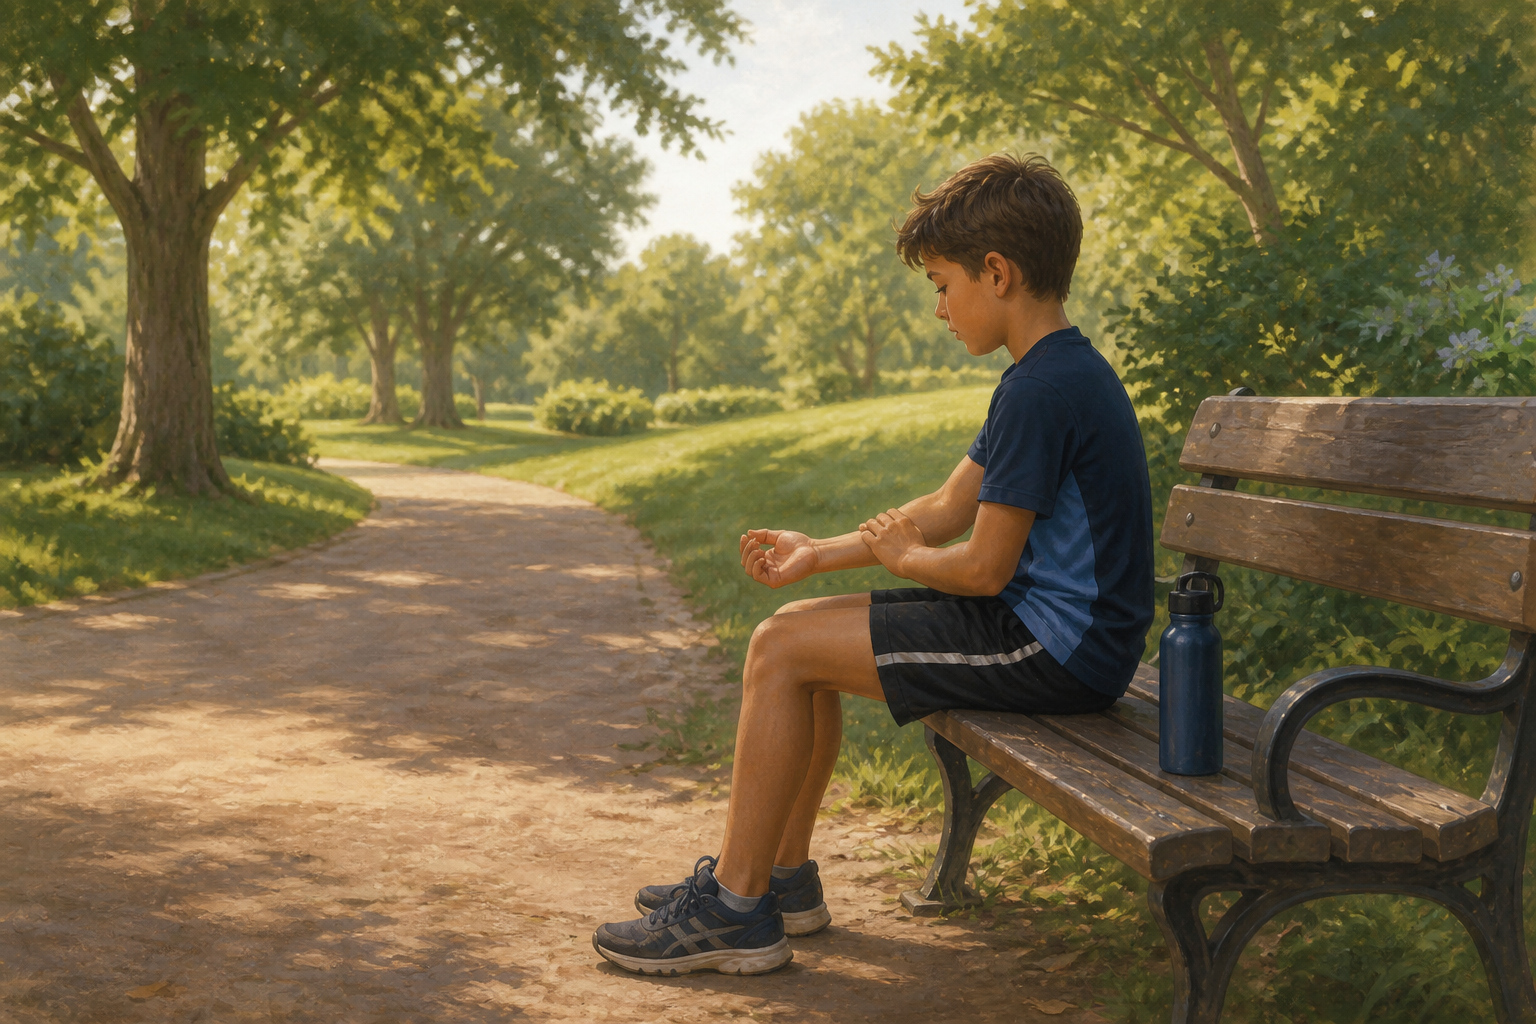
\includegraphics[width=0.58\linewidth]{images/book1/ai/g4-heart-rest.png}

{\small Depois da corrida: dois dedos no \omterm{prop:g4:heart-and-blood:pulse}{pulso}, contando a disparada
do \omterm{def:g4:heart-and-blood:heart}{coração} à distância.}
\end{omfigure}

\begin{remark}[Um músculo que nunca descansa --- quase]\label{rem:g4:heart-and-blood:rest}
Entre duas \omterm{def:g4:heart-and-blood:heart}{batidas} o \omterm{def:g4:heart-and-blood:heart}{coração} relaxa por uma fração de segundo ---
essa lasquinha é todo o descanso que ele tira. Dia e noite, cerca de
$100000$ \omterm{def:g4:heart-and-blood:heart}{batidas} por dia, a vida inteira. Como todo \omterm{def:g3:bones-and-muscles:muscle}{músculo}
(\cref{met:g3:bones-and-muscles:care}), ele fica mais forte com o
exercício: um \omterm{def:g4:heart-and-blood:heart}{coração} treinado move mais \omterm{prop:g4:journey-of-food:absorb}{sangue} por \omterm{def:g4:heart-and-blood:heart}{batida} e, por
isso, pode bater com mais calma.
\end{remark}

\section{Exercícios}

\begin{exercise}[$\star$]\label{exo:g4:heart-and-blood:1}
Diga duas coisas que o \omterm{prop:g4:journey-of-food:absorb}{sangue} entrega, e onde ele recolhe cada uma.
\end{exercise}

\begin{exercise}[$\star$]\label{exo:g4:heart-and-blood:2}
Que gás residual o \omterm{prop:g4:journey-of-food:absorb}{sangue} leva embora, e onde ele o deixa?
\end{exercise}

\begin{exercise}[$\star$]\label{exo:g4:heart-and-blood:3}
De que o \omterm{def:g4:heart-and-blood:heart}{coração} é feito, que tamanho ele tem e onde ele fica?
\end{exercise}

\begin{exercise}[$\star$]\label{exo:g4:heart-and-blood:4}
O que cada lado do \omterm{def:g4:heart-and-blood:heart}{coração} faz?
\end{exercise}

\begin{exercise}[$\star$]\label{exo:g4:heart-and-blood:5}
O que é o \omterm{prop:g4:heart-and-blood:pulse}{pulso}, e o que contar o \omterm{prop:g4:heart-and-blood:pulse}{pulso} diz a você?
\end{exercise}

\begin{exercise}[$\star$]\label{exo:g4:heart-and-blood:6}
Por que o \omterm{prop:g4:heart-and-blood:pulse}{pulso} deve ser medido com os dedos e não com o polegar?
\end{exercise}

\begin{exercise}[$\star$]\label{exo:g4:heart-and-blood:7}
Por que o \omterm{prop:g4:heart-and-blood:pulse}{pulso} dispara numa corrida? Conte a história do ponto de
vista dos \omterm{def:g3:bones-and-muscles:muscle}{músculos} das \omterm{def:g1:my-body:parts}{pernas}.
\end{exercise}

\begin{exercise}[$\star$]\label{exo:g4:heart-and-blood:8}
Faça a experiência: meça o seu \omterm{prop:g4:heart-and-blood:pulse}{pulso} em repouso com o
\cref{met:g4:heart-and-blood:pulse}, faça trinta segundos de
polichinelos e meça de novo. Informe os dois números.
\end{exercise}

\begin{exercise}[$\star\star$]\label{exo:g4:heart-and-blood:9}
No \cref{ex:g4:heart-and-blood:round}, a gota de \omterm{prop:g4:journey-of-food:absorb}{sangue} sai vermelha
viva dos pulmões e mais escura do \omterm{def:g3:bones-and-muscles:muscle}{músculo} da \omterm{def:g1:my-body:parts}{perna}. O que mudou
nela, em cada um dos casos?
\end{exercise}

\begin{exercise}[$\star\star$]\label{exo:g4:heart-and-blood:10}
O \omterm{prop:g4:journey-of-food:absorb}{sangue} liga três órgãos do seu ano: \omterm{def:g4:journey-of-food:tract}{intestino delgado}, pulmões,
\omterm{def:g4:heart-and-blood:heart}{coração}. Desenhe ou descreva a rede: o que cada um contribui para o
serviço de entregas?
\end{exercise}

\begin{exercise}[$\star\star\star$]\label{exo:g4:heart-and-blood:11}
O \omterm{prop:g4:heart-and-blood:pulse}{pulso} em repouso de um ciclista treinado pode ser $50$; o de um
adulto sem treino, $75$. Usando a
\cref{rem:g4:heart-and-blood:rest}, explique como \emph{mais lento}
pode querer dizer \emph{mais forte} --- o que cada \omterm{def:g4:heart-and-blood:heart}{batida} do ciclista
precisa estar fazendo?
\end{exercise}
